% !TeX spellcheck = pl_PL 
\chapter{Specyfikacja wewnętrzna}\label{chp:specWew}
\section{Struktura danych}
Reprezentację grafów w pamięci komputera można wykonać na dwa sposoby:
\begin{itemize}
	\item \textit{niskopoziomowy}: grafem jest macierz $ n\times n $ liczb całkowitych, gdzie $ n $ to liczba wierzchołków.\cite{id:AlgorytmyStruktury}
	\item \textit{wysokopoziomowy}: wierzchołki i łuki grafu są wyodrębnione do osobnych klas.
\end{itemize}
W pracy inżynierskiej zostało wybrane drugie podejście, zależności między klasami prezentuje rysunek \ref{fig:graphStructure}. Poprawne zdefiniowanie klas i zależności między nimi pozwala mi w intuicyjny sposób implementować algorytmy z pseudokodu: operacje rodzaju \textit{"wykonaj daną instrukcję na wszystkich łukach"} można łatwo odwzorować pobierając kolekcję krawędzi i dodając im odpowiednią metodę. Nie ma potrzeby adaptować operacji na zupełnie inną strukturę.
\begin{figure}[H]
	\centering
	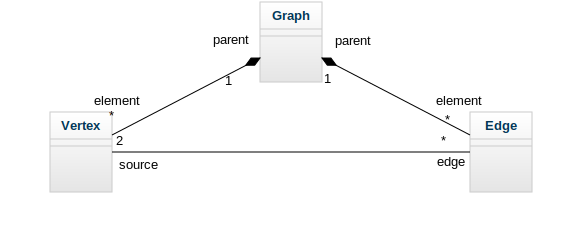
\includegraphics[width=0.6\textwidth]{./img/dane}
	\caption{Diagram klas struktury sieci}
	\label{fig:graphStructure}
\end{figure}
Zgodnie z definicją w \ref{ssec:graphDef}, graf (\emph{Graph}) składa się z dwóch zbiorów, wierzchołków (\emph{Vertex}) oraz łuków (\emph{Edge}). Graf jest kompozytem, wierzchołki i łuki stanowią jego ciało, a usunięcie obiektu grafu powoduje usunięcie jego wszystkich podrzędnych elementów. Wierzchołek jest niezależnym elementem, z kolei łuk posiada referencje do dwóch obiektów klasy wierzchołka - łuk nie może istnieć bez pary wierzchołków, które go tworzą, a usunięcie wierzchołka powoduje usunięcie wszystkich łuków wychodzących i wchodzących do niego.
\section{Konfiguracja wyglądu sieci}
Każdy obiekt sieci przepływowej posiada swoją konfigurację, w której znajdują się informacje dotyczące rysowania sieci. Każda sieć musi posiadać istniejącą konfigurację, jest to wymuszone poprzez jej konstruktor.
\begin{minted}
[
frame=lines,
framesep=2mm,
]{cpp}
explicit FlowNetwork(GraphConfig * config);
\end{minted}
Wierzchołki i łuki sieci przepływowej podczas wydarzenia rysowania pobierają swoje ustawienia z rodzica. Klasa \lstinline|GraphConfig| zawiera w sobie pięć składowych: nazwę sieci oraz cztery konteksty - sposób rysowania zwykłego elementu oraz zaznaczonego.\vfill
\cppcode{./listings/GraphConfig.cpp}
Informacje o sposobie rysowania wierzchołka są zawarte w klasie \mintinline{cpp}{VertexContext}, a łuki w klasie \mintinline{cpp}{EdgeContext}. Idea oparta jest o wzorzec \textbf{\textit{Pyłku}}. Każdy obiekt wierzchołka i łuku posiada swój niezmienny stan wewnętrzny, jak identyfikator oraz pozycję, a także stan zewnętrzny, jakim jest kolor i kształt\cite{id:WzorceProjektowe}. Kontekst oznacza właśnie stan zewnętrzny, którymi grafy mogą się różnić. Każdy wierzchołek i łuk posiada swój wskaźnik na aktualny kontekst, a w momencie, gdy następuje kliknięcie w element grafu i mechanizm \textit{Qt} wykrywa zmianę zaznaczenia, wskaźnik wskazuje na przeciwny kontekst.
\cppcode{./listings/itemChange.cpp}
\section{Serializacja sieci}\label{sec:serializacja}
Zapis oraz odczyt plików z grafami odbywa się w klasie \lstinline|GraphSerializer|. Posiada ona dwie publiczne metody:
\begin{itemize}
	\item \mintinline{cpp}{void serialize(GraphImage const & graph, std::string const & fileName);}\\
	Metoda \textit{serialize} przyjmuje jako parametr referencję do graficznej reprezentacji grafu, który ma zapisać oraz nazwę pliku wyjściowego wraz ze ścieżką.
	\item \mintinline{cpp}{GraphImage * deserialize(std::string const & filePath);}\\
	Metoda \textit{deserialize} przyjmuje jako parametr ścieżkę do pliku, który ma odczytać. Zwraca wskaźnik do graficznej reprezentacji grafu odczytanego z pliku.
\end{itemize}
Sieci przepływowe są zapisywane do formatu XML. W celu obsługi tego języka, klasa \lstinline|GraphSerializer| korzysta z darmowej biblioteki do parsowania plików XML, \emph{RapidXML}, autorstwa Marcina Kalicińskiego\footnote{Strona domowa \textit{RapidXML}: \url{http://rapidxml.sourceforge.net/}}
\subsection{Format pliku XML}
Plik zaczyna się od korzenia o nazwie \lstinline[language=XML]|<Graph>|. Format pliku można podzielić na dwie części, konfiguracyjną (gałąź \lstinline[language=XML]|<Config>|) i modelową (gałąź \lstinline[language=XML]|<Model>|). W pierwszej znajdują się globalne ustawienia wyglądu, jak rozmiary i kolory wierzchołków i łuków. Druga część zawiera model sieci przepływowej - zarówno pozycje i numery wierzchołków, jak i ich połączenia poprzez krawędzie, ich kierunek, przepustowość, przepływ oraz położenie napisu z informacją. Przykładowa sieć przepływowa oraz jej serializacja do pliku znajduje się w dodatku \ref{add:A}.\\\indent
Przy realizacji serializacji konieczne było zapewnienie sprawdzenia poprawności pliku. Jeżeli nie posiada poprawnego formatu XML lub brakuje danych do utworzenia sieci, aplikacja sygnalizuje błąd i nie tworzy nowej karty. Za każdym razem, gdy klasa \emph{GraphSerializer} potrzebuje w czasie deserializacji argumentu lub wartości, która nie istnieje w pliku XML, generowany jest wyjątek \lstinline[language=c++]|std::runtime_error| z odpowiednim komunikatem, który zostaje wyświetlony w nowym oknie dialogowym.


\section{Algorytmy}
Wszystkie trzy algorytmy wykonane w tej pracy zostały wyodrębnione do osobnych klas. Ich klasą bazową bazową jest \lstinline|FlowNetworkAlgorithm|, która definiuje interfejs algorytmów oraz zawiera wspólną dla wszystkich funkcjonalność.
\subsection{Tworzenie sieci residualnej}\label{ssec:tworzenieSieciResAlg}
Algorytm służący do wygenerowania sieci residualnej jest niezmienny dla wszystkich klas i jest zawarty w metodzie klasy \lstinline|FlowNetworkAlgorithm|.
\begin{minted}[
frame=lines,
framesep=2mm,
]{cpp}
int makeResidualNetwork(FlowNetwork * network, FlowNetwork *& outResidaulNetwork)
\end{minted}
Funkcja przyjmuje dwa parametry:
\begin{itemize}
	\item \emph{network} jest siecią przepływową na podstawie której jest utworzona sieć przepływowa
	\item \emph{outResidaulNetwork} jest referencją na wskaźnik do obiektu sieci, która będzie siecią residualną. W pierwszym kroku jest to głęboka kopia sieci przepływowej.
\end{itemize}
Wartością zwracaną jest najkrótsza odległość między źródłem, a ujściem, jeżeli tworzona sieć jest \textit{warstwową siecią residualną}. Jeżeli nie jest, funkcja zwraca zero. W pierwszym kroku, algorytm usuwa wszystkie łuki z wyjściowej sieci residualnej zostawiając same wierzchołki. Następnie przechodzi przez wszystkie łuki sieci przepływowej i wykonuje poniższy algorytm.
\begin{algorithm}
	\caption{Tworzenie nowego łuku w sieci residualnej}\label{siecResidualnaPseudo}
	\begin{algorithmic}
		\Procedure{Utwórz nowy łuk}{Łuk w sieci przepływowej}
			\State{Oblicz przepustowość residualną}
			\If{Istnieje łuk sąsiedni oraz łuk sąsiedni nie został odwiedzony}
				\State{Oblicz przepływy między wierzchołkami zgodnie z zachowaniem przepływu netto w \ref{ssec:netto}}
				\State Dodaj łuk oraz łuk sąsiedni do odwiedzonych
			\EndIf
			\If{Przepływ w łuku $\ne0$}
				\State{Utwórz nowy łuk w sieci residualnej w tym samym kierunku o przepustowości równej przepływowi}
			\EndIf
			\If{Przepustowość residualna $\ne0$}
				\State{Utwórz nowy łuk w sieci residualnej w przeciwnym kierunku o przepustowości równej przepustowości residualnej}
			\EndIf
		\EndProcedure
	\end{algorithmic}
\end{algorithm}
Utworzenie tablicy odwiedzonych łuków ma zapewnić, że w sieci residualnej nie zostaną utworzone nadmiarowe łuki gdy pętla dojdzie do sąsiada. Pełny kod algorytmu znajduje się dodatku \ref{add:B}.
\subsection{Szukanie ścieżki powiększającej}\label{ssec:szukanieSciezkiAlg}
Podczas realizacji algorytmów wymagane jest znalezienie pewnej ścieżki pomiędzy źródłem, a ujściem, jednak w literaturze (\cite{id:ZaawansowaneAlgorytmy},\cite{id:IntroductionToAlgorithms}) nie jest podany żaden konkretny sposób. Udowodniono, że wybór algorytmu do szukania ścieżki nie ma wpływu na wynik działania omawianych algorytmów - uzyskana wartość przepływu zawsze jest maksymalna. Zastosowano algorytm poszukiwania ścieżek własnego pomysłu, który został zaimplementowany w uogólnionej metodzie poszukującej drogi pomiędzy dwoma dowolnymi wierzchołkami sieci przepływowej.
\begin{minted}[
frame=lines,
framesep=2mm,
breaklines
]{cpp}
QList<EdgeImage*> FlowNetworkAlgorithm::findPathBetween(FlowNetwork * network, VertexImage * from, VertexImage * to)
\end{minted}
Funkcja przyjmuje trzy parametry:
\begin{itemize}
	\item \emph{network} jest siecią przepływową, która jest przeszukiwana.
	\item \emph{from} jest wierzchołkami startowym, z którego rozpoczynane jest szukanie ścieżki.
	\item \emph{to} jest wierzchołkiem docelowym, do którego dąży algorytm.
\end{itemize}
Wartością zwracaną jest lista wskaźników na łuki w sieci, która stanowi reprezentację znalezionej ścieżki. Jeżeli lista jest pusta, ścieżka między wierzchołkami nie istnieje.
\begin{algorithm}[H]
	\caption{Poszukiwanie ścieżki między wierzchołkami}\label{poszukiwanieSciezkiMiedzyWierzcholkami}
	\begin{algorithmic}
		\Procedure{Znajdź ścieżkę}{Sieć, wierzchołek startowy, wierzchołek docelowy}
			\State{Aktualnym wierzchołkiem jest startowy}
			\While{Szukanie się nie zakończyło}
				\ForAll{łuk wychodzący z aktualnego wierzchołka}
					\If{jeżeli łuk nie prowadzi do źródła, odrzuconego lub odwiedzonego wierzchołka}
						\State{Dodaj łuk do listy możliwych łuków}
					\EndIf
				\EndFor
				\If{lista możliwych łuków jest pusta}
					\If{ostatni łuk jest nullem}
						\Return{ścieżka}
					\Else
						\State{Dodaj aktualny wierzchołek do odrzuconych}
						\State{Usuń łuk z listy możliwych}
						\If{ścieżka nie jest pusta}
							\State{Cofnij się do poprzedniego wierzchołka}
						\Else
							\State{Aktualny łuk = null}\Comment{Aktualnym wierzchołkiem jest startowy}
						\EndIf
					\EndIf
				\EndIf
				\State{Wylosuj jeden z możliwych łuków}
				\State{Wierzchołek docelowy tego łuku jest aktualnym}
				\State{Dodaj aktualny wierzchołek do odwiedzonych}
				\State{Dodaj łuk do ścieżki}
				\State{Ostatnim łukiem jest aktualny}
				\If{aktualny wierzchołek jest docelowym}
					\State{zakończ algorytm}
				\EndIf
			\EndWhile\space
			\Return{ścieżka}	
		\EndProcedure
	\end{algorithmic}
\end{algorithm}
Algorytm jest bardzo prosty. Zaczynając od pierwszego wierzchołka, losowany jest jeden z jego łuków. Jeżeli łuk prowadzi do wierzchołka docelowego, koniec. Jeżeli nie, przechodzimy do tego wierzchołka i losujemy kolejny łuk, tak długo aż cel zostanie znaleziony. W przypadku gdy dalsza droga nie istnieje, następuje cofnięcie się do poprzedniego wierzchołka, aktualny wierzchołek oraz droga do niego zostają oznaczone jako odrzucone. Następnie losowany jest kolejny łuk z dostępnych, jeżeli już ich nie ma, następuje kolejne cofnięcie o wierzchołek. Jeżeli algorytm powróci do wierzchołka startowego, to ścieżka między wierzchołkami nie istnieje i zostaje zwrócona pusta lista. Aby algorytm nie odrzucił pierwszej pętli, sprawdzane jest dodatkowo czy ostatni wybrany łuk nie jest wartością null. Pełny kod algorytmu znajduje się dodatku \ref{add:findPathAlg}.\\\indent 
Dzięki swojej losowości, za każdym razem droga między wierzchołkami, wyznaczona przez program, będzie inna. Dzięki temu ścieżki powiększające i przepływy blokujące, w trakcie poszukiwania maksymalnego przepływu, również mogą się różnić przy rożnych wykonaniach algorytmu dla tej samej sieci. Nie ma tutaj jedynej słusznej drogi, jest jedynie jeden poprawny wynik.
\subsection{Zwiększenie przepływu w sieci}\label{ssec:zwiekszeniePrzeplywuAlg}
Algorytm zwiększania przepływu jest wspólny dla wszystkich algorytmów znajdowania maksymalnego przepływu.
\begin{minted}[
frame=lines,
framesep=2mm,
breaklines
]{cpp}
void FlowNetworkAlgorithm::increaseFlow(FlowNetwork *& network, QList<EdgeImage*> const & path, int increase)
\end{minted}
Funkcja przyjmuje trzy parametry:
\begin{itemize}
	\item \emph{network} jest siecią przepływową, gdzie przepływ zostanie zwiększony
	\item \emph{path} to zbiór łuków w których przepływ zostanie zwiększony
	\item \emph{increase} jest wartością o jaką przepływy zostaną zwiększone
\end{itemize}
\begin{algorithm}[H]
	\caption{Zwiększenie przepływu w sieci}\label{zwiekszenieParzeplywuAlg}
	\begin{algorithmic}
		\Procedure{Zwiększ przepływ}{Sieć, ścieżka, wartość powiększająca}
			\ForAll{łuk w ścieżce}
				\If{nie istnieje odpowiadający łuk w sieci}
					\State{Utwórz przepływ zwrotny w sąsiednim łuku}
				\ElsIf{istnieje odpowiadający łuk w sieci, ale posiada łuk sąsiedni}
					\State{Wykonaj optymalizację przepływu netto zgodnie z \ref{ssec:netto}}
				\Else\Comment{łuk istnieje i nie ma sąsiada}
					\State{Zwiększ przepływ w odpowiadającym łuku w sieci o wartość powiększającą}
				\EndIf
			\EndFor
		\EndProcedure
	\end{algorithmic}
\end{algorithm}
Algorytm musi uwzględniać trzy przypadki. Najprostszy występuje wtedy, gdy sieć posiada odpowiadający łuk, a ten nie posiada łuku sąsiedniego. Wówczas wystarczy jedynie zwiększyć przepływ. Jeżeli łuk posiada sąsiada, należy zwiększyć przepływ i dokonać wyrównania wartości. Może też zdarzyć się przypadek, że sieć residualna będzie posiadać łuki, które w sieci przepływowej nie istnieją, zgodnie z \ref{ssec:siecResidualna}. Wówczas należy dokonać przepływu zwrotnego, czyli zmniejszyć wartość przepływu w łuku, którzy dokonuje przepływu między wierzchołkami, ale w przeciwnym kierunku (który zgodnie z założeniami musi istnieć). Pełny kod algorytmu znajduje się dodatku \ref{add:increaseFlowAlg}.

\subsection{Warunki stopu}\label{ssec:warunkiStopu}
Poszukiwanie maksymalnego przepływu zostaje zakończone gdy zostanie spełniony jeden z warunków:
\begin{enumerate}
	\item Suma przepływów w łukach wychodzących ze źródła jest równa sumie ich przepustowości,
	\item Suma przepływów w łukach wchodzących do ujścia jest równa sumie ich przepustowości,
	\item Algorytm znajdowania ścieżki powiększającej [\ref{ssec:szukanieSciezkiAlg}] zwrócił pustą listę łuków.
\end{enumerate}
Pełna treść funkcji, które je sprawdzają znajdują się dodatku \ref{add:stopConditionsAlg}.

\subsection{Algorytm Forda-Fulkersona}\label{ssec:fordFulkersonWew}
Algorytm został zamknięty w klasie \emph{FordFulkersonAlgorithm}, która dziedziczy po \emph{FlowNetworkAlgorithm}. Pseudokod tego algorytmu znajduje się w rozdziale \ref{ssec:FordFulkersonAnaliza}. Jest to najprostsza z metod znajdowania maksymalnego przepływu i korzysta wyłącznie z metod odziedziczonych po klasie \emph{FlowNetworkAlgorithm}:
\begin{itemize}
	\item tworzenia sieci residualnej \ref{ssec:tworzenieSieciResAlg},
	\item znajdowania ścieżki powiększającej \ref{ssec:szukanieSciezkiAlg},
	\item zwiększania przepływu \ref{ssec:zwiekszeniePrzeplywuAlg}.
\end{itemize}
W pętli wykonywane są powyższe trzy instrukcje w kolejności w jakiej zostały wymienione. Efektem działania algorytmu jest sieć z maksymalnym przepływem. Pełny kod klasy tego algorytmu znajduje się dodatku \ref{add:fordFulkersonAlg}.
\subsection{Przepływ blokujący}\label{ssec:blockingFlowWew}
W klasie \emph{BlockingFlowAlgoritm} została zawarta cała logika związana z tworzeniem przepływu blokującego. Znajdują się tutaj wszystkie funkcje, które są wymagane do wykonania przepływu. Zgodnie z teorią zawartą w \ref{ssec:blockingFlowAnaliza} do wykonania przepływu blokującego potrzebna jest informacja o odległościach pomiędzy wierzchołkiem źródłowym, a wszystkimi pozostałymi. Informacja ta jest przechowywana w macierzy liczb zmiennoprzecinkowych $ n\times n $, gdzie $ n $ to liczba wierzchołków.
\begin{minted}[
frame=lines,
framesep=2mm, tabsize=4,
]{cpp}
typedef std::vector<std::vector<float>> FloatMatrix;
class BlockingFlowAlgoritm
{
protected:
	FloatMatrix _pathMatrix;
}
\end{minted}
Z kolei do wyznaczenia odległości między wierzchołkami został wykorzystany algorytm Floyda-Warshalla \cite{id:AlgorytmyStruktury}, który wyszukuje odległości między wszystkimi parami wierzchołków. W sieci przepływowej odległość między wierzchołkami połączonymi przez łuk jest równa jeden. Implementacja funkcji znajduje się w dodatku \ref{add:floydWarshallImpl}.

\subsection{Algorytm Dinica}\label{ssec:dinicAlgWew}
Algorytm został zwarty w klasie \emph{DinicAlgorithm} dziedziczącej po klasach \emph{FlowNetworkAlgorithm} oraz \emph{BlockingFlowAlgoritm}. Implementacja tego algorytmu różni od implementacji algorytmu Forda-Fulkersona \ref{ssec:fordFulkersonWew} tworzeniem sieci residualnej, która jest warstwowa. W efekcie klasa tworzy sieć residualną metodą odziedziczoną po \emph{FlowNetworkAlgorithm}, a następnie usuwa zbędne elementy w metodzie odziedziczonej po \emph{BlockingFlowAlgoritm}.
\begin{minted}[
frame=lines,
framesep=2mm, tabsize=4,breaklines,
]{cpp}
int DinicAlgorithm::makeResidualNetwork(FlowNetwork * network, FlowNetwork *& residualNewtork)
{
	FlowNetworkAlgorithm::makeResidualNetwork(network, residualNewtork);
	return removeRedundantElements(residualNewtork);
}
\end{minted}
Funkcja \emph{removeRedundantElements} usuwa z przekazanej sieci residualnej nadmiarowe elementy. W tym celu pobiera z tablicy \lstinline{_pathMatrix} (\ref{ssec:blockingFlowWew}) potrzebne wartości i porównuje je zgodnie z  warunkami opisanymi w \ref{ssec:WSR}. Pełna treść tej funkcji znajduje się w dodatku \ref{add:removeRedundantElements}.\\\indent
Algorytm Dinica wykorzystuje wyszukiwanie ścieżki powiększającej do zwiększania przepływów w warstwowej sieci residualnej. Po utworzeniu przepływu blokującego, który na początku każdej iteracji jest głęboką kopią warstwowej sieci residualnej, wyszukiwane są w nim wszystkie istniejące ścieżki powiększające z wykorzystaniem algorytmu opisanego w \ref{ssec:szukanieSciezkiAlg}. Uzyskane ścieżki zapisuje się do wektora ścieżek powiększających, a na koniec realizuje je wszystkie zwiększając przepływ w taki sam sposób jaki opisano w \ref{ssec:zwiekszeniePrzeplywuAlg}, z tą tylko różnicą, że wykonuje się je w pętli. Kod tego procesu został przedstawiony w dodatku \ref{add:blockPrzeplywZapel}.
\subsection{Algorytm MKM}
Ten algorytm wykorzystuje pojęcie potencjału przepływowego \ref{ssec:mkmAnaliza}, więc jego klasa wymaga utworzenia dodatkowej składowej. Do każdego wierzchołka należy dodać informację o jego trzech potencjałach (wejściowym, wyjściowym i ogólnym), więc wykorzystano strukturę \lstinline|std::tuple|. Wartościami są liczby zmiennoprzecinkowe, które umożliwiają stosowanie nieskończoności (\lstinline|std::numeric_limits|).
\begin{minted}[
frame=lines,
framesep=2mm, tabsize=4,breaklines,
]{cpp}
typedef QMap<int, std::tuple<float, float, float>> PotentialMap;
class MkmAlgorithm : public FlowNetworkAlgorithm, public BlockingFlowAlgoritm
{
	PotentialMap _potentialMap;
}
\end{minted}
Mapa potencjałów, gdzie kluczem jest id wierzchołka, jest aktualizowana w każdej iteracji, natychmiast po utworzeniu warstwowej sieci residualnej. Ta klasa wymagała gruntowanej zmiany zwiększania przepływu w przepływie blokującym: w każdej iteracji najpierw musi wyszukać wierzchołek o najmniejszym potencjale, z niego poprowadzić dwie ścieżki, do źródła oraz do ujścia, jak również sprawdzić nowy warunek stopu. W aplikacji jest to zrealizowane w następujący sposób:
\begin{algorithm}[H]
	\caption{Tworzenie przepływu blokującego algorytmem MKM}\label{mkmZwiekszeniePrzeplywuAlg}
	\begin{algorithmic}
		\Procedure{Znajdź ścieżkę powiększającą}{Sieć $ G_f^w $, referencja na przepustowość residualną $ c $}
		\Repeat
			\State{Wyczyść obie ścieżki}
			\State{Znajdź nieodrzucony wierzchołek $ v $ o najmniejszym, niezerowym potencjale w sieci $ G_f^w $}
			\If{jeżeli taki wierzchołek nie istnieje}
				\State{Wyjdź z pętli}
			\EndIf
			\State{Znajdź ścieżkę z wierzchołka $ v $ do ujścia $ t $}
			\State{Znajdź ścieżkę ze źródła $ s $ do wierzchołka $ v $}
			\If{jedna ze ścieżek jest pusta}
				\State{Odrzuć wierzchołek}
			\Else
				\State{$ c= $ potencjał wierzchołka $ v $}
				\State{Zwiększ maksymalny przepływ o $ c $}
			\EndIf
		\Until{ścieżka ze źródła = 0 lub ścieżka do ujścia = 0}
		\State{\Return{suma ścieżki ze źródła i ścieżki do ujścia}}
		\EndProcedure
	\end{algorithmic}
\end{algorithm}
Dwie ścieżki, ze źródła do wierzchołka i z wierzchołka do źródła, jakie zostały opisane w definicji algorytmu (\ref{ssec:mkmAnaliza}), tak naprawdę tworzą razem pojedynczą ścieżkę powiększającą. W implementacji zostało to wykorzystane i w każdej iteracji zwracana jest suma obu zbiorów - tworzona jest pojedyncza ścieżka o jednej przepustowości residualnej. Dzięki temu nie było potrzeby ani zmiany interfejsu ani skorzystania ze wzorca Adaptera.\\\indent
Algorytm wykonywany jest tak długo aż zostanie znaleziona ścieżka przepływowa, czyli jest droga ze źródła do ujścia prowadzącą przez wierzchołek $ v $. Algorytm kończy swe poszukiwanie również wtedy jeżeli nie istnieje wierzchołek, który miałby niezerowy potencjał. Po każdej iteracji uzyskana ścieżka dodawana do jest listy ścieżek powiększających wraz ze swoją przepustowością residualną, tak jak w implementacji algorytmu Dinica \ref{ssec:dinicAlgWew}.\\\indent
Wierzchołkami odrzuconymi są te znalezione wierzchołki, przez które nie prowadzi żadna ścieżka powiększająca. Mogą takie się znaleźć w warstwowej sieci residualnej i są dodawane do listy odrzuconych, by nie przechodzić przez nie w kolejnych iteracjach. Pełna treść tej procedury znajduje się w dodatku \ref{add:mkmImpl}.